\section{Gaussian Cluster Demo}

To illustrate the theoretical relationship between Gaussian clusters and linear separators with absolute value activation functions, we conducted a simple demonstration using 2D Gaussian data. This demo compares the behavior of single-layer neural networks using Absolute Value (Abs) and Rectified Linear Unit (ReLU) activation functions when learning to approximate the Mahalanobis distance of points in a 2D Gaussian cluster.

\subsection{Experimental Setup}

The demonstration consists of the following key components:

\begin{itemize}
    \item \textbf{Data Generation:} We create a 2D Gaussian cluster with a specified mean and covariance matrix, calculating the true Mahalanobis distance for each point.
    \item \textbf{Models:} Two single-layer neural networks are implemented, one with Abs activation and one with ReLU, both trained to predict the Mahalanobis distance of input points.
    \item \textbf{Training:} Models are trained using Stochastic Gradient Descent (SGD) optimizer for a specified number of epochs.
    \item \textbf{Visualization:} We plot log-scale error curves for both models, scatter plots of the Gaussian cluster, and visualizations of learned model parameters.
\end{itemize}

\subsection{Results and Analysis}

Our experiments revealed two distinct scenarios for the Abs model, highlighting the complex dynamics of neural network training even in simple cases.

\subsubsection{Ideal Case: Abs Aligns with Gaussian Structure}

In the ideal scenario, the Abs model successfully aligns its weight vector with the principal axis of the Gaussian cluster, as predicted by our theoretical analysis.

\begin{figure}[H]
    \centering
    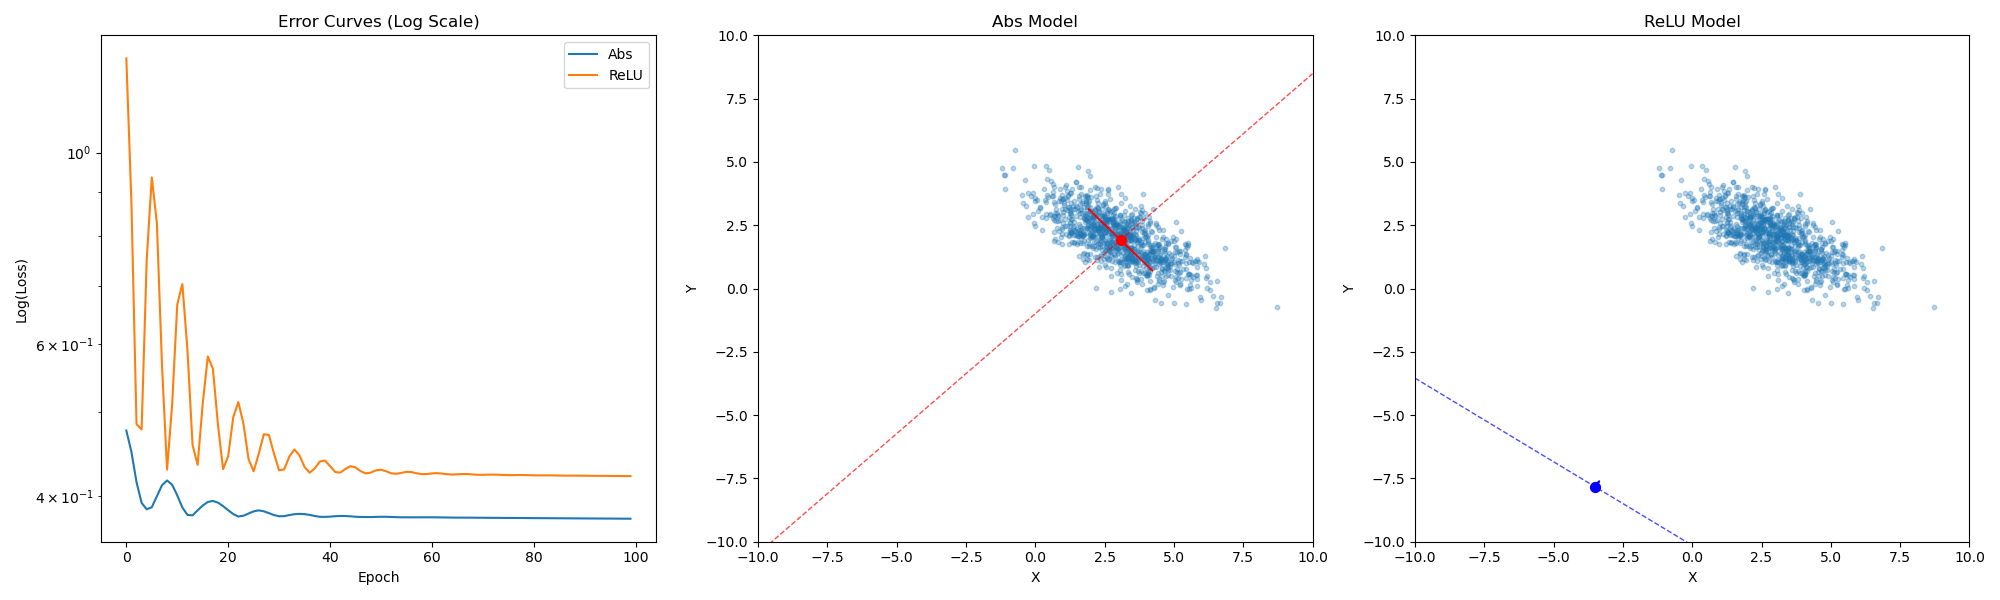
\includegraphics[width=\textwidth]{img/demo1_ideal.png}
    \caption{Ideal case: Abs model aligns with Gaussian structure}
    \label{fig:ideal_case}
\end{figure}

Figure \ref{fig:ideal_case} illustrates this case. Key observations include:

\begin{itemize}
    \item The Abs model's weight vector (red lines) aligns closely with the principal axis of the Gaussian cluster.
    \item The ReLU model positions itself to approximate the Mahalanobis distance from one side, resulting in a less accurate representation of the Gaussian structure.
    \item The error curve shows the Abs model achieving lower final error compared to the ReLU model.
\end{itemize}

This result demonstrates the potential of Abs activation to implicitly learn and represent the structure of Gaussian clusters, aligning with our theoretical predictions. In contrast, the ReLU model's solution, while potentially achieving a low error, does not reflect a grounded representation of the data's underlying structure. The ReLU model merely positions itself to approximate the Mahalanobis distance from one side, essentially finding a shortcut that works for this specific data distribution but lacks the structural insight captured by the Abs model.

This distinction is crucial: while the ReLU solution may perform adequately on the given dataset, it fails to capture the inherent symmetry and full dimensional structure of the Gaussian cluster. As a result, the ReLU model's solution is less likely to generalize well to new data or slight variations in the input distribution. It's not overfitting in the traditional sense, but rather a form of superficial learning that doesn't encapsulate the true nature of the data.

The Abs model's alignment with the principal component, on the other hand, represents a more fundamental understanding of the data's structure. This grounded representation is more likely to generalize robustly and provide meaningful insights about the underlying data distribution, aligning closely with the theoretical relationship between Gaussian clusters and linear separators with absolute value activations.

\subsubsection{Suboptimal Case: Abs Falls into Local Minimum}

In some instances, the Abs model falls into a local minimum similar to the ReLU solution, deviating from the theoretically optimal alignment.

\begin{figure}[H]
    \centering
    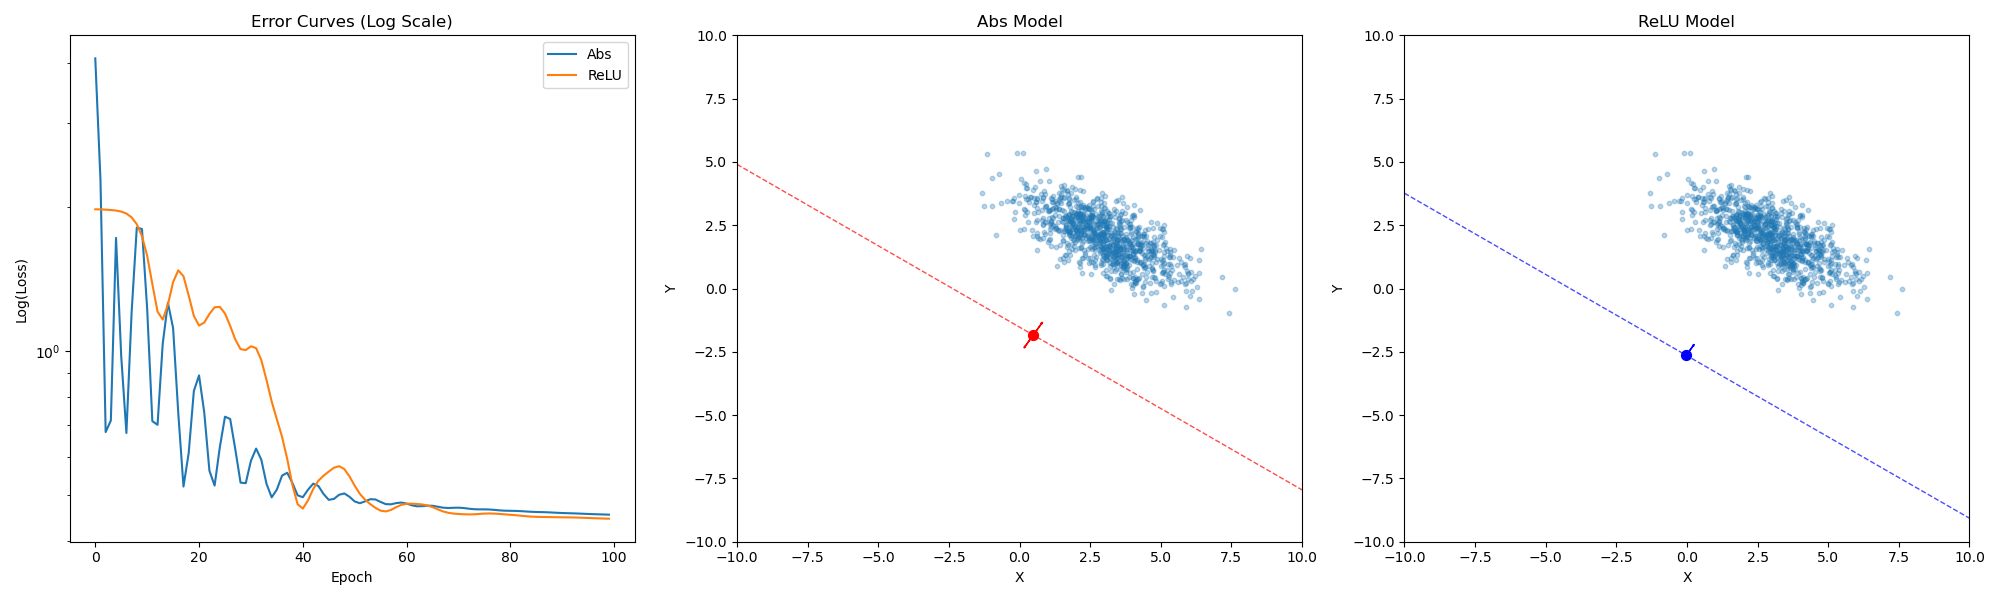
\includegraphics[width=\textwidth]{img/demo1_suboptimal.png}
    \caption{Suboptimal case: Abs model falls into local minimum}
    \label{fig:suboptimal_case}
\end{figure}

Figure \ref{fig:suboptimal_case} shows this scenario. Notable observations:

\begin{itemize}
    \item The Abs model's weight vector does not align with the principal axis of the Gaussian cluster.
    \item Both Abs and ReLU models adopt similar positions, approximating the Mahalanobis distance from one side.
    \item In this case, the ReLU model achieves slightly lower final error.
\end{itemize}

This suboptimal case highlights the challenges in consistently achieving theoretically optimal solutions in practice, emphasizing the importance of initialization and optimization strategies in leveraging the potential advantages of Abs activations.

\subsection{Implications and Future Directions}

These results provide valuable insights into the behavior of Abs activation functions in the context of Gaussian data structures:

\begin{itemize}
    \item They demonstrate the potential for Abs activations to implicitly learn Gaussian cluster representations, as predicted by our theoretical analysis.
    \item The occurrence of suboptimal solutions highlights the complexity of neural network training dynamics, even in simple scenarios.
    \item These observations motivate further research into initialization techniques and optimization strategies to consistently achieve theoretically optimal solutions with Abs activations.
\end{itemize}

As we extend our investigation to more complex architectures and datasets, these insights will guide our understanding of how the theoretical advantages of Abs activations manifest in practical deep learning scenarios.